\part{Analyse de l'existant}
\thispagestyle{part}
\parttoc

	\chapter{Blackfire}
	\label{chap:Blackfire}
		\section{Architecture générale}
			% Schéma :  https://d2vqbs7xgyce6n.cloudfront.net/assets/v44abae9bcb/bundles/blackfire/img/general-workflow.png
			% Pour chaque composant : rôle/objectifs/problématiques... (Agent / Sonde / API / Companion)
			% En commentaire du schéma montrant comment ils s'organisent entre eux
	
\begin{figure}[!h]
\begin{center}
  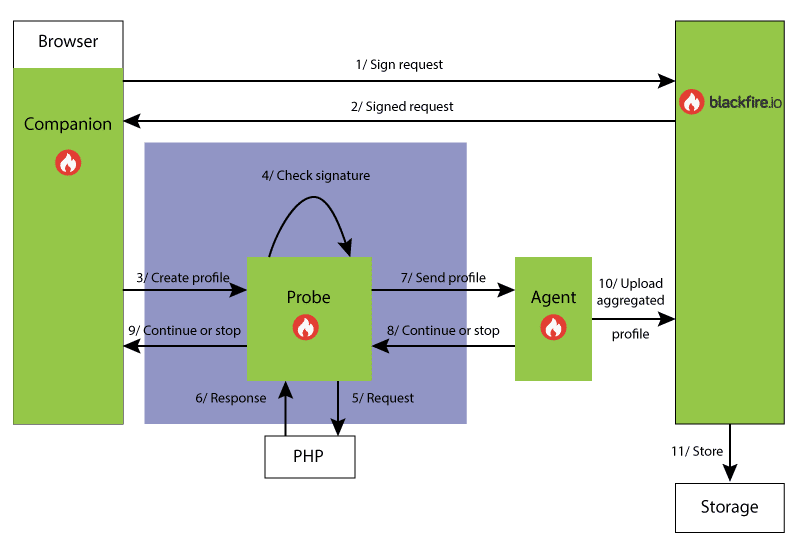
\includegraphics[width=0.8\textwidth]{images/schemas/workflow/general-workflow}
  \caption{Fonctionnement général de \Blackfire}
\end{center}
\end{figure}

Ce graphique montre comment les quatre composants de \Blackfire interagissent entre eux lors de l'établissement d'un profil.
 
Ainsi, on commence par le \textbf{compagnon}. Son rôle est de générer la requête\footnote{Voir section \vref{subsec:BlackfireQuery}} en communiquant avec le site blackfire.io, de l'envoyer à la sonde, puis d'afficher un retour à l'utilisateur sur le statut de son profil : y a-t-il eu une erreur ? et sinon, quels sont les coûts principaux\footnote{On parle ici des temps du nœud racine, main, également appelés coûts d'enveloppe.} ?

Ensuite, une fois que la \textbf{sonde} a reçu la requête, celle-ci va la vérifier, instrumenter le code de l'application, analyser ce dernier et générer le profil correspondant. Le profil est ensuite envoyé à l'agent\footnote{Voir section \vref{subsec:comm-agent}} qui retourne un statut que la sonde retransmet au compagnon\footnote{Voir section \vref{subsec:comm-compagnon}}. Le rôle de la sonde est donc d'instrumenter le code, de générer le profil puis de l'envoyer à l'agent.

Une fois que l'\textbf{agent} a reçu le profil, il va le vérifier et le pré-traiter, entre autres pour anonymiser certains arguments de fonction comme les requêtes SQL, qui sont susceptibles de contenir des informations sensibles. Puis il va envoyer ce profil au site blackfire.io.

Enfin, le site \textbf{blackfire.io}\footnote{Aussi appelé API par la suite} a pour rôle de stocker et d'afficher les profils aux utilisateurs.

		\section{Protocole}
			\label{sec:BlackfireProtocol}
			% Retour sur certains éléments du protocole
Pour faire communiquer les différents composants entre eux, \Blackfire utilise un protocole textuel répondant à quatre objectifs principaux :
\begin{itemize}
\item Authentifier une demande de profil
\item Fournir les informations nécessaires pour générer le profil
\item Transmettre le profil généré
\item Fournir un retour à l'utilisateur
\end{itemize}

			\subsection{La Requête}
			\label{subsec:BlackfireQuery}
				% émise par le companion ou l'outil CLI via run/curl
				% pas de détail sur la signature ou le contenu précis de la requête. On se contente de ce que l'on va utiliser plus tard
La requête, émise par le client\footnote{Via l'utilisation du compagnon par exemple}, permet à la fois d'authentifier une demande de profil et de fournir à la sonde un certain nombre d'options de configuration relatives au profil à générer.

Pour cela, la requête est composée de deux parties:
\begin{itemize}
\item Une série d'arguments accompagnée d'une signature cryptographique qui permet d'authentifier la demande et d'en vérifier la validité
\item Une série d'options de configuration permettant d'activer ou de désactiver certaines parties de la sonde\footnote{Par exemple l'option \verb?flag\_cpu? permet de désactiver la collecte des temps CPU}.
\end{itemize}

			\subsection{Communication avec le compagnon}
			\label{subsec:comm-compagnon}
				% Y a-t-il autre chose que le Blackfire-Response: continue ici ? Expliquer l'enjeu et l'importance de cet en-tête
L'un des usages de \Blackfire est de profiler, à l'aide du compagnon, une page web servie par un serveur distant. Dans ce cas, tout se déroule sur le serveur distant et l'utilisateur n'a aucun moyen de consulter ce qui est produit durant l'analyse. Par conséquent il est important de fournir au compagnon un retour indiquant si le profil a été généré. Cette réponse, générée par l'agent, est ensuite retransmise par la sonde au compagnon en définissant l'en-tête \verb|X-Blackfire-Response| dans la réponse \emph{HTTP}.

			\subsection{Communication avec l'agent}
			\label{subsec:comm-agent}
				% Format du hello prolog
				% La réponse de l'agent (avec les fn args)
L'analyse est déclenchée par le compagnon mais elle est réellement gérée par l'agent. Pour cela il existe un protocole en deux étapes\footnote{NB: Le protocole a évolué dans une version récente de \Blackfire avec l'introduction du fichier \verb?.blackfire.yml?} entre la sonde et l'agent.

La première étape consiste à faire authentifier la requête par l'agent\footnote{En réalité l'agent n'authentifie pas la requête mais demande à l'API de le faire}. Pour cela, la sonde commence par envoyer deux en-têtes à l'agent. Le premier, \verb|Blackfire-Query|, contient la partie signée de la requête (et la signature) afin que l'agent la valide. Le second, \verb|Blackfire-Probe|, permet d'identifier la technologie instrumentée.

\begin{listing}[H]
\caption{En-têtes envoyés à l'agent par la sonde}
\begin{textcode}
Blackfire-Query: <requête>
Blackfire-Probe: python-20706f0
\end{textcode}
\end{listing}
Ici, l'en-tête \verb|Blackfire-Probe| indique que l'on analyse du python en version 34014960 (tel que défini par \mintinline{python}{hex(sys.hexversion)}\footnote{\url{https://docs.python.org/2/library/sys.html#sys.hexversion}}).

La seconde partie consiste en une réponse envoyée par l'agent et contenant une ligne de statut. En cas d'erreur, celle-ci est de la forme \verb|Blackfire-Error: <code> <raison>| et est destinée à être journalisée par la sonde. Sinon, elle est de la forme \verb|Blackfire-Response:| \verb|<message>| et est destinée à être retransmise telle quelle au compagnon. En plus du statut, l'agent peut aussi renvoyer des informations identifiant des fonctions dont on désire récupérer les arguments. Ces informations se trouvent sous la forme d'une série de lignes ayant le format suivant: \verb|Blackfire-Fn-Args: <fonction> <argument>|,
\verb|<fonction>| étant le nom de la fonction à instrumenter (tel qu'affichée dans le graphe) et \verb|<argument>| le nombre d'arguments à récupérer.

Par exemple les lignes suivantes indiquent qu'il faut récupérer le premier argument de la fonction \verb|logging.error| et les deux premiers arguments de la méthode \verb|log| de la classe \verb|logging.error|
\begin{listing}[H]
\caption{En-têtes définissant les arguments de fonction à récupérer}
\begin{textcode}
Blackfire-Fn-Args: logging.error 1
Blackfire-Fn-Args: logging.Logger::log 2
\end{textcode}
\end{listing}

				\subsection{Format des profils}
					% cf: http://blog.blackfire.io/blackfire-file-format.html
\Blackfire utilise un format textuel\footnote{Voir Annexe \vref{app:fullProfile} pour un exemple complet de profil} pour décrire les profils générés après l'analyse d'un programme.

Un profil est composé de deux sections séparées par une ligne vide. La première définit un certain nombre d'en-têtes décrivant le contexte du profil. Ainsi les principaux en-têtes sont:
\begin{itemize}
\item \verb|file-format: BlackfireProbe| qui définit le format utilisé, celui-ci ayant évolué au cours du temps\footnote{La sonde \PHP actuelle ainsi que la sonde \Python utilisent le format \emph{BlackfireProbe}}
\item \verb|graph-root-id: <nom>| qui définit le nom du point d'entrée du programme analysé
\item \verb|cost-dimensions: <liste>| qui définit la liste des dimensions envoyées par la sonde (temps wall-time, cpu, consommation mémoire...). Les dimensions sont séparées par des espaces
\item \verb|probed-os: <os>|, \verb|probed-language: <langage>|, \verb|probed-version: <langage version>| qui permettent de définir l'environnement d'exécution du programme.
\end{itemize}

La seconde section définit le \gls{graphe d'appels} du programme. Celui-ci est construit à partir de ses arcs, une ligne correspondant à un arc.

\begin{listing}[H]
\caption{Ligne de profil simple (pas d'argument de fonction)}
\begin{textcode}
<appelant>==><appelé>//<coûts>
\end{textcode}
\end{listing}

\begin{itemize}
\item \verb|<appelant>| est le nom du nœud appelant
\item \verb|<appelé>| est le nom du nœud appelé
\item \verb|<coûts>| est la liste des coûts pour le lien. Les coûts sont séparés par des espaces et correspondent aux dimensions définies précédemment.
\end{itemize}

	\chapter[Analyse en \Python]{Analyse de performances en \Python}
Il existe différents outils et API permettant d'analyser les performances ou le comportement d'un code \Python, et on peut regrouper ces outils en deux catégories : ceux qui fonctionnent en mode \gls{SaaS} (comme \emph{Blackfire}) et ceux qui fonctionnent de manière indépendante ou sont directement intégrés dans \emph{Python}.

		\section{Outils tiers existants}
Il existe plusieurs outils tiers permettant de s'intéresser au fonctionnent d'une application \Python et parmi ceux-là l'un d'entre eux va nous occuper : \emph{New Relic\footnote{\url{https://www.newrelic.com}}}. %et \emph{Opbeat\footnote{\url{https://www.opbeat.com}}}.

			\subsection{New Relic}
          		\begin{wrapfigure}{r}{0.5\textwidth}
  \vspace{-30pt}
  \begin{center}
    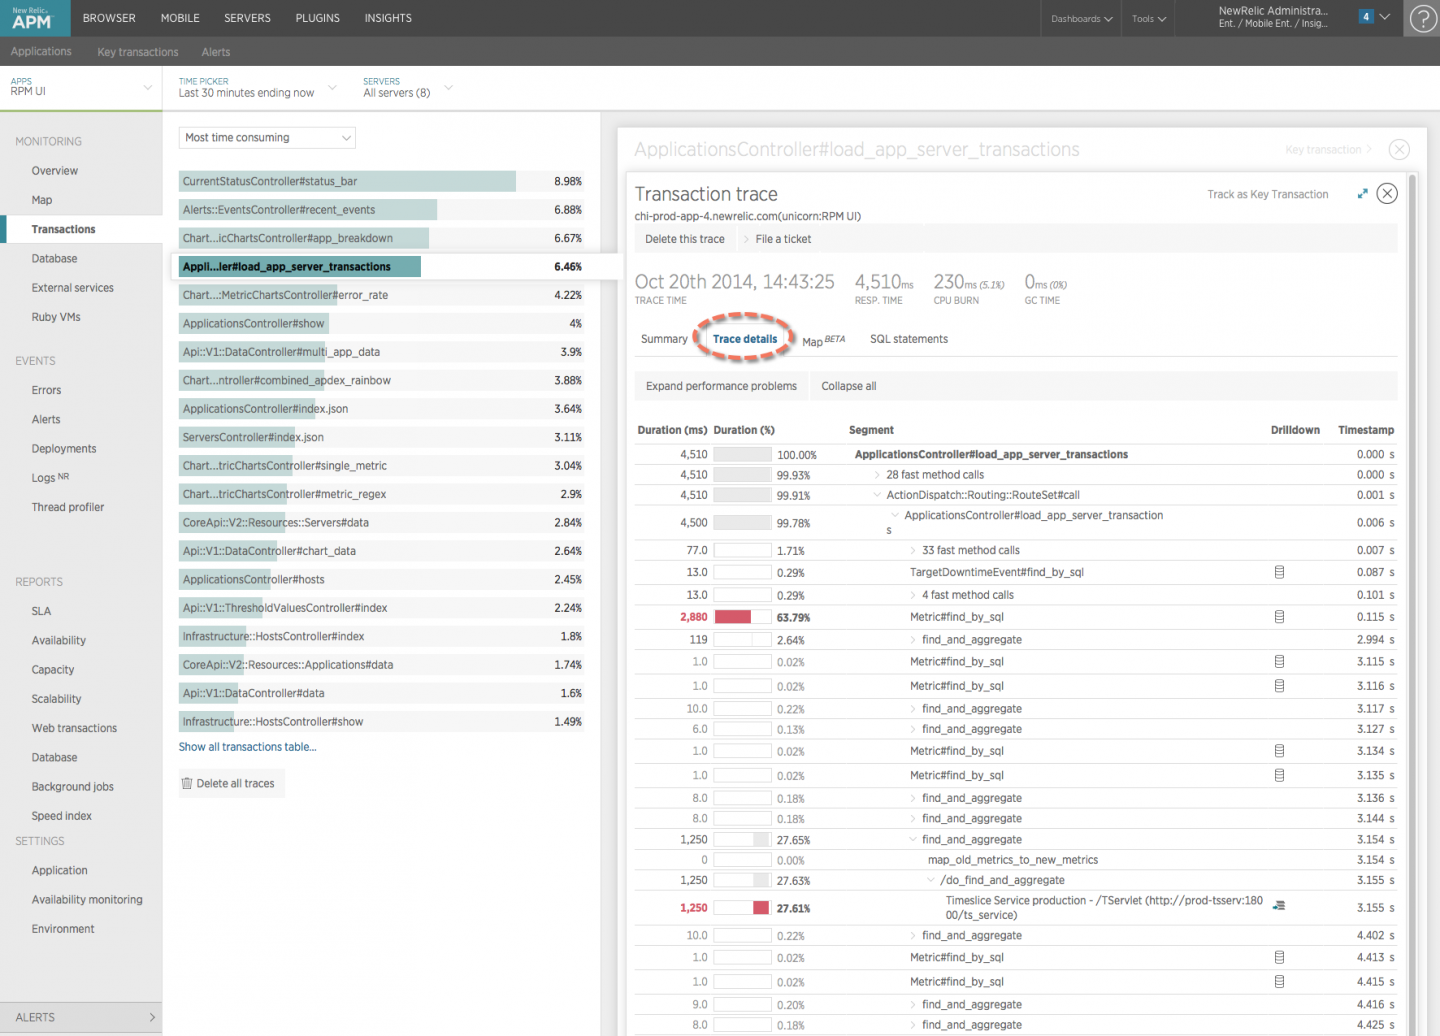
\includegraphics[width=0.48\textwidth]{images/new-relic_trace}
  \end{center}
  \vspace{-22pt}
  \caption{\emph{New Relic} - exemple de trace}
  \vspace{-20pt}
\end{wrapfigure}

\emph{New Relic} est un outil disponible en mode \gls{SaaS} permettant de monitorer les serveur de \gls{production} tout en ayant un impact sur les performances négligeable.

Ils proposent différentes fonctionnalités dont notamment une permettant d'afficher, sous forme de trace, des métriques sur le code exécuté. Il va ainsi permettre d'afficher une trace, un profil du code exécuté avec le temps passé dans chaque fonction.
 
\clearpage
Cet outil est intéressant sur plusieurs points :
\begin{itemize}
  \item Le langage \Python est supporté
  \item L'expérience utilisateur est proche de celle de \Blackfire (pas ou peu d'instrumentation manuelle de requise)
\end{itemize}
  
Enfin le code source du module de l'agent \emph{New Relic} pour \Python est disponible sur \gls{PyPI}\footnote{\url{https://pypi.python.org/pypi/newrelic}} ce qui permet de comprendre son fonctionnement.
  
  \subsubsection{Collecte des métriques}
Pour collecter le graphe d'appels et les temps associés deux techniques semblent être en œuvre :
Tout d'abord l'agent va lancer un thread spécial qui sera chargé de récupérer la \gls{pile d'appels} à intervalle régulier et de l'utiliser pour reconstituer le \gls{graphe d'appels} du programme.
 
En parallèle diverses méthodes et fonctions estimées importantes sont décorés afin de récupérer plus d'information comme le temps d'exécution ou la requête SQL exécutée.

Cette instrumentation se fait en plusieurs étapes \footnote{Voir Annexe \vref{app:newrelicdecorationmethodes} pour le code correspondant} :
\begin{enumerate}
  \item Définition d'un \emph{\gls{chargeur de module}} personnalisé afin de décorer automatiquement les modules quand ils sont chargés.
  \item Lecture dans le fichier de configuration de la liste des méthodes à décorer.
  \item Enregistrement d'un \emph{\gls{hook}} pour chacune des méthode à décorer auprès du chargeur de module.
  \item Lors du chargement d'un module, le chargeur de module va exécuter tous les hooks se rapportant au module en question afin d'en décorer les méthodes.
\end{enumerate}

Cette instrumentation fonctionne à partir d'un fichier de configuration indiquant quelles méthodes doivent être instrumentées, elle est donc parfaitement générique. En outre le fait de n'instrumenter qu'une partie des appels de fonctions permet de l'imiter l'impact du profileur au point d'en être négligeable, surtout qu'il existe une librairie\footnote{\url{https://pypi.python.org/pypi/wrapt}} (écrite dans le langage C) permettant de décorer facilement et à moindre coup n'importe quelle fonction ou méthode \Python.

En revanche cette technique impose de connaître et d'indiquer à l'avance la liste exhaustive des fonctions intéressantes.

  \subsubsection{Expérience utilisateur}
			%\subsection{Optbeat}
			%	  \subsubsection{Présentation}
  \subsubsection{Fonctionnalités}
  \subsubsection{Fonctionnement}
			
		\section{Python}
			%\subsection{Pycallgraph}
			%\label{subsec:pycallgraph}
			%	\input{existant/python-python-pycallgraph} 
			%\subsection{Pyinstrument}
			%\label{subsec:pyinstrument}
			%	\input{existant/python-python-pyinstrument}
			\subsection{Python C-Profiler / \textunderscore lsprof} 
			\label{subsec:cprofiler}
				\Python fournit trois modules\footnote{\url{https://docs.python.org/2/library/profile.html}} permettant d'analyser les performances d'un programme et de générer des rapports à partir des données collectées. Ils utilisent tous les trois la même technique, à savoir l'utilisation de \verb|sys.setprofile()|\footnote{\verb?sys.setprofile()? ayant la particularité d'être intégré directement dans le cœur de \Python et d'accepter n'importe quelle fonction de rappel, qu'elle soit écrite en \C ou en \Python - Voir \url{https://docs.python.org/2/library/sys.html#sys.setprofile} pour plus de détails} pour définir une fonction de rappel qui est appelée à chaque fois que l'interpréteur entre ou sort d'une fonction. L'événement \verb|CALL|\footnote{Lancé quand l'interpréteur entre dans une fonction} permettant de récupérer le nom de la fonction et de relever la date\footnote{La date est relevée de la manière la plus précise possible, la résolution restant néanmoins dépendante du système sur lequel l'application tourne} lorsque celle-ci au début de la fonction, et l'événement \verb|RETURN|\footnote{Lancé quand l'interpréteur sort d'une fonction} permettant de mesurer la date en sortie de la fonction, de calculer la différence entre le début et la fin de cette dernière et de stocker le résultat.

De plus ces trois modules collectent les mêmes données, à savoir les temps exclusif\footnote{En excluant le temps passé dans les autres fonctions} et inclusif\footnote{En incluant le temps passé dans les autres fonctions} passés dans chaque fonction et le nombre de fois qu'elle a été appelée. De plus ils génèrent leur rapport dans le même format, à savoir \verb|pstat|\footnote{\url{https://docs.python.org/2/library/profile.html#module-pstats}}, mais ils ont néanmoins de grandes différences d'implémentation et ne servent pas le même usage : 

\begin{itemize}
\item \textbf{cProfile} est le module recommandé dans la majorité des cas, il s'agit d'une extension \C ayant un impact sur les performances relativement limité.
\item \textbf{profile} est un module écrit en pur \Python et ayant exactement la même interface que le \emph{cProfile}. Par contre son impact sur les performances est très important, mais étant écrit en \Python il est plus facile de le modifier et de l'étendre.
\item \textbf{hotshot} est un autre module écrit en \C. A la différence du \emph{cProfile} son objectif est d'avoir un impact sur les performances le plus faible possible, quitte à devoir passer plus de temps dans une phase de post-traitement. En revanche il n'est plus maintenu aujourd'hui et a été supprimé dans \Python 3.
\end{itemize}
			\subsection{Yappi}
			\label{subsec:yappi}
				\emph{Yappi}\footnote{\url{https://bitbucket.org/sumerc/yappi}}, pour \emph{Yet Another Python Profiler}, est un logiciel open source\footnote{Sous licence \emph{MIT}} créé en 2009 par \emph{Sümer Cip} et permettant d'analyser les performances d'un programme \emph{Python}.

Il s'agit d'un module écrit en \C utilisant le même fonctionnement que le \emph{C-Profiler}, dont il est inspiré (à savoir l'utilisation d'une fonction de rappel qui est appelée à chaque fois que l'on entre ou sort d'une fonction).

D'un point de vue fonctionnel, \emph{Yappi} a été conçu de manière à avoir un impact sur les performances de l'application mesurée le plus faible possible, et dispose de quelques fonctionnalités qui ne sont pas présentes dans le \emph{C-Profiler} :
\begin{itemize}
\item Possibilité d'avoir des temps CPU à la place des temps utilisateur
\item Gestion du multi threading
\begin{itemize}
\item Les threads sont automatiquement analysés
\item Les appels de fonction des différents threads ne sont pas différenciés (on ne peut pas savoir quel thread a effectué un appel de fonction donné) 
\item Le temps total passé dans chaque thread est disponible
\end{itemize}
\end{itemize}
				
				
				
				
				
				
				
				
				
				
				
				
				
				
				
				
				
				
				
				
				
				
				
				
				
				
				
				
				
				
				
				
				